% ==========================================================================================
% Dissertation template and document class for Princeton University
% Author  : Jeffrey Scott Dwoskin <jdwoskin@princeton.edu>
% Adapted from: http://www.math.princeton.edu/graduate/tex/puthesis.html
% ==========================================================================================

%%-- For print copies
%% set 'singlespace' option to set entire thesis to single space, and define "\printmode" to remove all hyperlinks for printed copies of the thesis. Delete all output files before changing this mode -- it will turn hyperref package on and off
%\documentclass[12pt,lot, lof, singlespace]{puthesis}
%\newcommand{\printmode}{}

%%-- For the electronic copy, use doublespacing, define "\proquestmode" to use outlined links, instead of colored links.
\documentclass[12pt,lot, lof]{puthesis}
\newcommand{\proquestmode}{}
% I prefer proquestmode to be off for electronic copies for normal use, since the colored links are less distracting. However when printed in black and white, the colored links are difficult to read.

%%-- For early drafts without some of the frontmatter
% Also see the "ifodd" command below to disable more frontmatter
%\documentclass[12pt]{puthesis}

%%---- Author & title page info ----%%
\title{Recombination X-Ray Laser Based on Ionization-recombination Mechanism of Atomic Excitation}

\submitted{July 2011}  % degree conferral date (January, April, June, September, or November)
\copyrightyear{2011}  % year in which the copyright is secured by publication of the dissertation.
\author{Chao LU}
\adviser{Professor Marlan O. Scully}  %replace with the full name of your adviser
%\departmentprefix{Program in}  % defaults to "Department of", but programs need to change this.
\department{Mechanical Engineering}

%%---- Tweak float placements ----%%
% From: http://mintaka.sdsu.edu/GF/bibliog/latex/floats.html "Controlling LaTeX Floats"
% and based on: http://www.tex.ac.uk/cgi-bin/texfaq2html?label=floats
% LaTeX defaults listed at: http://people.cs.uu.nl/piet/floats/node1.html

%%-- Alter some LaTeX defaults for better treatment of figures:
%% See p.105 of "TeX Unbound" for suggested values.
%% See pp. 199-200 of Lamport's "LaTeX" book for details.
%% General parameters, for ALL pages:
    \renewcommand{\topfraction}{0.85}	% max fraction of floats at top
    \renewcommand{\bottomfraction}{0.6}	% max fraction of floats at bottom
%% Parameters for TEXT pages (not float pages):
    \setcounter{topnumber}{2}
    \setcounter{bottomnumber}{2}
    \setcounter{totalnumber}{4}     % 2 may work better
    \setcounter{dbltopnumber}{2}    % for 2-column pages
    \renewcommand{\dbltopfraction}{0.66}	% fit big float above 2-col. text
    \renewcommand{\textfraction}{0.15}	% allow minimal text w. figs
%% Parameters for FLOAT pages (not text pages):
    \renewcommand{\floatpagefraction}{0.66}	% require fuller float pages
	% N.B.: floatpagefraction MUST be less than topfraction !!
    \renewcommand{\dblfloatpagefraction}{0.66}	% require fuller float pages

%% The documentclass already sets parameters to make a high penalty for widows and orphans.


%%---- Use packages ----%%
%\usepackage{amsfonts}
\usepackage{amssymb}
\usepackage{amsmath}

%%-- For figures
\usepackage{graphicx}
%\usepackage{subfig,rotate}

%%-- For comments
\usepackage{verbatim}

%%-- For tables
\usepackage{multirow}
%% Longtable lets you have tables that span multiple pages.
\usepackage{longtable}

%% Booktabs produces far nicer tables than the standard LaTeX tables.
%% See: http://en.wikibooks.org/wiki/LaTeX/Tables
\usepackage{booktabs}

%% Set parameters for longtable:
%% default caption width is 4in for longtable, but wider for normal tables
\setlength{\LTcapwidth}{\textwidth}


%%---- Printed vs. online formatting ----%%
\ifdefined\printmode        % Printed copy

%% Url package understands urls (with proper line-breaks)
%% but without hyperlinking them.
\usepackage{url}

\else

\ifdefined\proquestmode        %ProQuest copy

%% Proquest requirements: http://www.princeton.edu/~mudd/thesis/Submissionguide.pdf
%% ProQuest requires a double spaced version (set previously).
%% They will take an electronic copy, so we want links in the pdf.
%% But also copies may be printed or made into microfilm in black and white,
%% so we want outlined links instead of colored links.
\usepackage{hyperref}
\hypersetup{bookmarksnumbered}

%% copy the already-set title and author to use in the pdf properties
\makeatletter
\hypersetup{pdftitle=\@title,pdfauthor=\@author}
\makeatother

\else        %Online copy

%% Adds internal linked references, pdf bookmarks, etc.
%% Turn all references and citations into hyperlinks:
%% - Not for printed copies.
%% - Automatically includes url package.
%% Options:
%%  colorlinks makes links by coloring the text instead of putting a rectangle around the text.
\usepackage{hyperref}
\hypersetup{colorlinks,bookmarksnumbered}

%% Copy the already-set title and author to use in the pdf properties
\makeatletter
\hypersetup{pdftitle=\@title,pdfauthor=\@author}
\makeatother

%% Make the page number rather than the text be the link for ToC entries
%\hypersetup{linktocpage}
\fi %Proquest or online formatting
\fi %Printed or online formatting


%%---- Define commands ----%%

%% Define any custom commands that you want to use.
%% For example, highlight notes for future edits to the thesis:
%% \newcommand{\todo}[1]{\textbf{\emph{TODO:}#1}}

%% Create an environment that will indent text.
%% See: http://latex.computersci.org/Reference/ListEnvironments
%%   \raggedright makes them left aligned instead of justified
\newenvironment{indenttext}{
    \begin{list}{}{ \itemsep 0in \itemindent 0in
    \labelsep 0in \labelwidth 0in
    \listparindent 0in
    \topsep 0in \partopsep 0in \parskip 0in \parsep 0in
    \leftmargin 1em \rightmargin 0in
    \raggedright
    }
    \item
  }
  {\end{list}}

%% Another environment that's an indented list, with no spaces between items
%% -- if we want multiple items/lines. Useful in tables.
%%  Use \item inside the environment.
%%  \raggedright makes them left aligned instead of justified
\newenvironment{indentlist}{
    \begin{list}{}{ \itemsep 0in \itemindent 0in
    \labelsep 0in \labelwidth 0in
    \listparindent 0in
    \topsep 0in \partopsep 0in \parskip 0in \parsep 0in
    \leftmargin 1em \rightmargin 0in
    \raggedright
    }

  }
  {\end{list}}

%%---- Front-matter ----%%
%% For early drafts, you may want to disable some of the frontmatter.
%% Simply change this to "\ifodd 1" to do so.
\ifodd 0

%% Front-matter disabled while writing chapters.
\renewcommand{\maketitlepage}{}
\renewcommand*{\makecopyrightpage}{}
\renewcommand*{\makeabstract}{}

%% you can just skip the \acknowledgements and \dedication commands to leave out these sections.

\else
\abstract{
%% Abstract can be any length, but should be max 350 words for a Dissertation
%% for ProQuest's print indicies (150 words for a Master's Thesis)
%% or it will be truncated for those uses.
\abstract{Chemical kinetics and fluid dynamics are crucial components of combustion, governing the efficiency, stability, and emissions of many practical combustion devices.  Particularly, this dissertation advances the understanding of the coupling effects between chemical kinetics and transport in flame dynamics (Chapters~\ref{ch:NTC} and~\ref{ch:dynamics}) and soot emissions (Chapters~\ref{ch:biofuel} and~\ref{ch:bluff}) at engine relevant conditions.  For both topics, foundational studies on chemical kinetics were first carried out in relatively simple, laminar, low-dimensional configurations with well characterized flow fields to understand low-temperature cool flame chemistry and soot chemistry.  Complexities from flows were then considered, and chemistry-transport coupling was investigated at engine relevant conditions to elucidate the role of low-temperature chemistry in autoignition-affected flame dynamics and the role of hydrogen addition in soot evolution in bluff body flames, leveraging the understanding obtained in the chemical kinetics studies.  

The first half of this dissertation focuses on low-temperature chemistry and its role in flame dynamics.  Specifically, in Chapter~\ref{ch:NTC}, experimental studies, supported by computations, were conducted on the coupling of low-temperature chemistry and transport in the ignition, extinction, and associated steady burning in nonpremixed DME/air counterflow flames.  The presence of low-temperature chemical reactivity was detected nonintrusively, and the ignition temperature was determined subsequently.  At elevated pressures, which promote low-temperature chemistry, the hysteresis in ignition and extinction behavior of nonpremixed cool flames was observed and quantified for the first time.  The thermal and chemical structure of the cool flame was computationally analyzed to elucidate the dominant chemical pathways during the ignition and extinction processes.  Effects of strain rate, fuel and oxygen concentration, and ambient pressure on the cool flame were investigated.  Possible reasons for the discrepancies between experiments and computations were discussed to facilitate further cool flame studies and the development of low-temperature chemical models.

The role of low-temperature chemistry in autoignition-affected flame dynamics was then computationally investigated in Chapter~\ref{ch:dynamics}.  Laminar nonpremixed DME/air coflow flames were investigated at elevated temperatures and pressures with various boundary temperatures and velocities.  The stabilization mechanism for steady flames and the flame dynamics for the forced oscillating cases were analyzed.  Besides the tribrachial structure typically observed at nonautoignitive conditions, a multibrachial thermal structure was observed due to autoignition.  Consequently, a stabilization regime diagram was proposed, including frozen flow, kinetically stabilized (autoignition), autoignition-propagation-coupled stabilized, kinematically stabilized (tribrachial flame), and burner stabilized regimes.  The transition of the combustion mode was elucidated through the computational investigations of sinusoidally forced oscillating cases.  Transition between a multibrachial autoignition front and a tribrachial flame occurs periodically and exhibited a hysteresis.  First-stage low-temperature chemistry is less affected by flow dynamics with only second-stage autoignition and flame chemistry, which accounts for the majority of the heat release, coupled with flow oscillation.  The understanding of the role of low-temperature chemistry in flame dynamics under laminar autoignitive conditions lays the foundation for future studies at turbulent conditions in practical engines. 

The second half of this dissertation focuses on soot emissions.  To understand the fuel effects on soot chemistry, in Chapter~\ref{ch:biofuel}, the sooting limits of nonpremixed $n$-heptane, $n$-butanol, and methyl butanoate flames were determined experimentally in a liquid pool stagnation-flow configuration.  In addition, complementary simulations with detailed polycyclic aromatic hydrocarbon (PAH) chemistry and a detailed soot model, based on the Hybrid Method of Moments (HMOM), were performed and compared with the experimental critical strain rates for the sooting flames.  Argon dilution was used to keep the thermal environment for the three fuel cases nearly the same to elucidate the chemical effects.  Both experiment and simulation showed that $n$-heptane and $n$-butanol had similar sooting characteristics, while methyl butanoate had the least sooting propensity.  Further sensitivity and reaction pathway analysis demonstrated that the three fuels share similar PAH chemical pathways, and C$_5$ and C$_6$ ring formation from the intermediate chain species was found to be the rate-limiting step.  The differences in sooting propensity were due to the role of fuel bounded oxygen and the fuel breakdown processes.  The findings in this chapter provide guidance to the design of diesel/biofuel blendings to reduce soot emissions.

Finally, in Chapter~\ref{ch:bluff}, the evolution of soot in a turbulent nonpremixed bluff body ethylene/hydrogen flame was investigated using a combination of experiments and Large Eddy Simulations and compared with a neat ethylene counterpart.  With hydrogen addition, the maximum soot volume fractions in the recirculation zone and jet-like region significantly decreased.  Flamelet calculations demonstrated that hydrogen addition suppressed soot formation due to the reduction of the C/H ratio, resulting in an estimated fourfold reduction in soot volume fraction due to chemical effects.  Soot reduction in the downstream jet-like region of the flame was quantitatively consistent with this chemical effect.  However, soot reduction in the recirculation zone was substantially larger than this analysis suggests, indicating an additional hydrodynamic effect.  Large Eddy Simulation was used to further investigate soot evolution in the recirculation zone and to elucidate the role of hydrogen addition.  For the same heat release rate and similar jet Reynolds number as the neat ethylene case, the addition of hydrogen required a higher jet velocity, and this led to a leaner recirculation zone that inhibited soot formation and promoted soot oxidation.  The findings in this chapter further validated the comprehensive soot model for turbulent sooting flames and advanced the understanding of soot evolution in recirculating flows.} 


}

\acknowledgements{
%I would like to thank...
I would like to thank the Math department for providing the original documentclass file that this class is based upon. I would like to thank my parents, without whom my life would not be possible. I would also like to thank my advisor, my dissertation committee, and my research collaborators because every graduate student needs to do so. And finally, I thank the members of my research group, to whom I leave this template to save you some of the trouble I had to go through getting my dissertation to compile in \LaTeX{}.  

Don't forget to ask your advisor if your work was sponsored by a grant that needs to be acknowledged in this section.  
}

\dedication{To my parents.}

\fi  %disable frontmatter


%%-- Hide some chapters

%% If you want to produce a pdf that includes only certain chapters, specify them with includeonly,
%% in addition to including all chapters below.
%\includeonly{ch-intro/chapter-intro}

%% You can also specify multiple chapters.
%\includeonly{ch-intro/chapter-intro,ch-usage/chapter-usage}
%\includeonly{chap1,chap2,chap3}


%%-- Notes:
%% Footnotes should be placed after punctuation.\footnote{place here.}
%% Generally, place citations before the period~\cite{anotherauthor}.
%% The proper usage for i.e., and e.g., include commas ``(e.g., option A, option B)''

%%---- Text ----%%
\begin{document}
\makefrontmatter

%% If you've disabled frontmatter, you can insert the toc manually.
%\tableofcontents\clearpage

%% \include lets us split up the document (and each include starts a new page):
\chapter{Introduction\label{ch:intro}}

\section{Recombination X-ray}
It is as early as the 1970's, the gain of recombination scheme of
X-ray lasers is predicted, by scientist from Soviet Union. But this
scheme is verified experimentally until 1985, by Szymon Suckewer,
who observed X-ray radiation at the wavelength of $18.2nm$, from
Carbon 3->2 transition. Then he made another breakthrough at 1993, in
Lithium, where the lasing between 2->1 is realized. The signification
is that it is the first experiment achieved lasing to ground state.

Recent news that X-ray free electron laser at SLAC (Stanford) became
operational at $0.15$ nm provided tremendous excitement for scientists in
various disciplines. Very large efforts made by many researchers, engineers
and technicians over a dozen of years at a very substantial cost is finally
paying off. The very large cost of such a large \textquotedblleft scientific
tool\textquotedblright\ did not diminish the importance of the achievement,
which is expecting to have a profound impact on the studies in many fields
such as crystallography, and condense matter, in general, and high
resolution microscopy of biological elements, etc. in particular. However,
very large cost and size, resulting in low flexibility regarding the use of
this important device has forced researchers to search for a more portable,
less expensive XUV and X-ray devices, which can be used in individual
researchers laboratories for preparatory work before going into these larger
facilities.

In particular, a portable X-ray laser operating in a transient regime at $%
13.5$ nm has been demonstrated in Suckewer's group \cite{Koro96} (see Fig. %
\ref{Li}). The laser uses H-like Li ions as an active medium which are
excited by ionization-recombination process in a microcapillary. The
excitation mechanism is the following. First, a strong $250$ $fs$ laser
pulse (power density 10$^{17}$W/cm$^{2}$) creates nonequilibrium plasma of Li%
$^{3+}$ ions and electrons. Electron density is $10^{19}-10^{20}$ cm$^{-3}$.
The ion-electron recombination occurs on a time scale faster then $1$ ps
which creates Li$^{2+}$ (H-like) ions in highly excited states (large
principle quantum number $n$). By collisions atoms are transferred to states
with smaller $n$ on a few ps time scale. For proper density population
inversion between the level $n=2$ and the ground state ($n=1$) is created
for $10-100$ ps. This results in lasing on the wavelength of the $n=2$ to $%
n=1$ transition ($13.5nm$) which is measured by a spectrometer. Experimental
setup and the measured spectrum is shown in the figure \ref{Li}.

As demonstrated in the figure \ref{Li}, a low power $2$ Hz Nd/YAG laser ($100
$ mJ$,$ $5ns$) was focused with an $f/6$ lens on the entrance of
microcapillary. Microcapillaries of lengths from $1$ to $5$ $mm$ and
diameters of $0.3$ $mm$ were made in solid LiF by drilling appropriate
holes. After a few hundred nsec delay (varied between 300 and 1000 ns), the
Ti:sapphire $250$ $fs$ laser was fired, whose energy is $50-60$ mJ in a
repetition rate $2$ Hz. This femto-second laser was tightly focused with the
same $f/6$ lens onto the plasma at the entrance of the microcapillary
providing a power density close to $2\times 10^{17}$ $W/{cm}^{2}$. The
Nd/YAG laser beam was directed to the microcapillary by a near
100reflectivity mirror, $M_{1}$, and the femto-second laser beam was
directed by directed by a mirror, $M_{2}$ which is transparent for the $1.06$
$\mu m$ wavelength of the Nd/YAG laser. From the output spectra, we could
see the soft X-ray lasing.

In the present research we are trying to make a laser in a similar way,
however, instead of ions, we want to use neutral He atoms which are easier
to confine then plasma. Fig. \ref{He} shows He energy level diagram and
radiative decay times for various transitions. We want to make a laser
operating at the $2~^{1}$P $\rightarrow 1~^{1}$S transition ($58$ nm). So,
we need to create population inversion between those levels. We are planning
to do it in two stages. First, we populate the triplet $2~^{3}$S
state by ionization-recombination processes similar to what has been done in
the Li-ions experiment. Then we transfer population into the singlet $2~^{1}$
P state of He by sending short optical laser pulses which yields population
transfer via the triplet $3~^{3}$D state.

\subsection{Preparation of orthohelium}
First we inject an ultrashort high power laser pulse to ionize the He gas.
Then we turned off the laser and rapid recombination and de-excitation
follow such that the lowest states of He atoms are prepared according to
their statistical weights. Hence for the sake of simplicity we take the
relative population of the triplet $2~^{3}\text{%S}$ and singlet $1~^{1}\text{%
  S}$ states to be 3 to 1.

Let me consider the physics of the laser plasma as produced in our Princeton
lab. We envision a laser plasma created by Keldysh tunneling with a non
Boltzmann distribution of neutral excited atoms. This involves $\text{He}%
^{++}\rightarrow \text{He}^{+}\rightarrow \text{He}$ electron capture via
three-body recombination. Three-body recombination for H-like ions is
approximately proportional to the forth power of the principal quantum
number $n^{4}$ and to the square of the electron density as ${N_{e}}^{2}$.
Hence for sufficiently high initial electron density three-body
recombination will dominate radiative decay.

However, the collisional ionization from highly excited states is also fast,
thus in order for three-body recombination rates to dominate ionization
rates, the recombining plasma should have a low electron temperature $\text{T%
}_{e}$. For example, for $k_{B}\text{T}_{e}\approx 1$ $eV$, initial electron
density $N_{e}\approx 2\times 10^{16}$ cm$^{-3}\approx N_{\text{He}^{++}}$
for fully ionized $\text{He}^{++}$ in quasi-neutral plasma, the equilibrium
between recombination and ionization processes will be established after a
few dozen picoseconds at a ratio of $N_{e}/N_{\text{He}}\approx 3\times
10^{-3}$ for $N_{\text{He}}=10^{16}$ cm$^{-3}$. This ratio becomes even
smaller ($N_{e}/N_{\text{He}}\approx 10^{-8}$) for $k_{B}\text{T}_{e}\approx
0.5$ $eV$. In such way one can obtain an essentially neutral gas of excited
He atoms.

In order to create a fully ionized $\text{He}^{++}$ plasma at low
temperature, we consider the example of a plasma capillary 10-100 $\mu $m in
diameter and a few cm long. The tunneling ionization can be used to generate
the plasma \cite{Keld65,Burn89,avi04,avi07}. In this way one can strip both
electrons from He atoms without significantly heating the plasma, especially
for ultra-short laser pulses. The laser intensity needs to be in the order
of $10^{16}$ W/cm$^{2}$ for efficient tunneling ionization of He to $\text{He%
}^{+}$ and to $\text{He}^{++}$ according to Keldysh theory \cite{Keld65}.
For needle like plasma column such intensities can easily be obtained from a
Ti/Sapphire laser at wavelength $\lambda =0.8$ $\mu $m with $\sim $ $10$ mJ
energy per pulse in pulses of $50-100$ fs duration with ionization pulse
propagating in plasma channel. Use of such short pulses is crucial to
minimize plasma heating. It is important to use laser pulses shorter than
collision times of electrons in order to minimize plasma heating during the
ionization process.

The bottom line is that we can create a cold laser plasma which recombines
to produce an excited neutral gas. In particular the metastable triplet $%
2~^{3}\text{S}$ (8000 s radiative life time) state will be formed with a
statistical weight of around 3 compared to the $1^{1}\text{S}$ state. The
population in the $2~^{3}\text{S}$ state is then transferred to the $3~^{3}%
\text{D}$ state via the $2~^{3}\text{P}$ levels by dark state adiabatic
transfer (STIRAP).

\subsection{Population transfer from $2~^{3}\text{S}$ to $3~^{3}$D via STIRAP
  process}

Robust population transfer from the triplet $2~^{3}\text{S}$ to triplet $%
3~^{3}\text{D}$ is then made possible by Stimulated Raman Adiabatic Passage
(STIRAP) \cite{Berg98}. In this technique one subjects the system, whose
state is $2~^{3}\text{S}$ at $t=0$, to a so called counter intuitive pulse
sequence with Rabi frequencies $\Omega _{1}$ and $\Omega _{2}$ in which the $%
\Omega _{1}$ ($2~^{3}\text{P}\rightarrow 3~^{3}\text{D}$) pulse precedes the
$\Omega _{2}$ ($2~^{3}\text{S}\rightarrow 2~^{3}\text{P}$) pulse. This pulse
sequence ideally results in a complete transfer of population to the desired
state $3~^{3}\text{D}$ without necessarily populating the $2~^{3}\text{P}$
state in the process.

The mechanism of STIRAP is best understood in the dressed state basis in
which we introduce bright and dark states. Beginning with the dark state
\begin{equation}
  |0~\rangle =\frac{\Omega _{1}|2~^{3}\text{S}\rangle -\Omega _{2}|3~^{3}\text{%
      D}\rangle }{\sqrt{\Omega _{1}^{2}+\Omega _{2}^{2}}}
\end{equation}%
we apply $\Omega _{1}$ before $\Omega _{2}$ so that $|0\rangle \cong |2^{3}%
\text{S}\rangle $ during the early stages of transfer. Then we adiabatically
turn on $\Omega _{2}$ while turning off $\Omega _{1}$, such that $|0\rangle
\cong |3~^{3}\text{D}\rangle $ for large times. The condition of
adiabaticity implies the following estimate of the required pulse energy
(see Appendix A)

\begin{equation}
  W\gtrsim 1000\frac{\hbar cS}{\lambda ^{3}\gamma \tau _{\text{pulse}}},
  \label{s3a}
\end{equation}%
where $S$ is the cross section area of the pulse, $\tau _{\text{pulse}}$ is
the pulse duration, $\lambda $ and $\gamma $ are the wavelength and the rate
of the transition. For the weakest 2$^{3}$P$\rightarrow $2$^{3}$S transition
$\lambda =1083$ nm and $\gamma =10^{7}$s$^{-1}$. Then for a plasma capillary
of radius $\sim 0.1$mm and pulse duration $\tau _{\text{pulse}}=1$ ps Eq. (%
\ref{s3a}) yields $W\gtrsim 20$ $\mu \text{J}$. Currently pico-second lasers
are commercially available with much greater energy.

\subsection{Population transfer from $3~^{3}\text{D}$ to $2~^{1}$P: level degeneracy problem}

Once the population is transferred to the $3~^{3}\text{D}$ state a strong
resonant driving field is applied on the $3~^{3}\text{D}$ to $2~^{1}\text{P}$
transition. However, levels $3~^{3}$D and $3~^{1}$D are essentially
degenerate (splitting between them is $0.2$ nm) and the applied external
field inevitably drives transition $3~^{1}\text{D}$ to $2~^{1}$P which is
more then 1000 times stronger then $3~^{3}$D to $2~^{1}$P transition (see
Fig. \ref{He}). Thus, the Rabi frequency which drives the $3~^{1}$D to $%
2~^{1}$P transition is much larger then those driving the $3~^{3}$D to $%
2~^{1}$P transition. Under such condition, practically no population can be
transferred from the $3~^{3}$D state as shown in Fig. \ref{f1}. This is true
no matter how strong the driving field is.

To avoid this problem it has been suggested to apply an additional resonant
field which drives the $3~^{1}\text{D}$ to $4~^{1}\text{P transition. The
  equivalent scheme is sketched in the insert of Fig. }$\ref{f2}. If the
additional driving field $\Omega _{bc}(t)$ is strong enough the population
can be transferred completely from $3~^{3}\text{D}$ to $2~^{1}\text{P (see
  Fig. }$\ref{f2}). The condition for an efficient population transfer is that
the amplitude $A$ of the additional field Rabi frequency $\Omega _{bc}(t)$
is greater then those of $\Omega _{cd}(t)$. This is demonstrated in Fig. \ref%
{f3} which shows population transfer as a function of $A$.

Result shown in the figures are obtained by numerical solution of the
evolution equations for $C_{a}$, $C_{b}$, $C_{c}$ and $C_{d}$ which are
probability amplitudes to find the system in the states $a$, $b$, $c$ and $d$
respectively. For resonant driving fields the evolution equations read%
\begin{equation}
  \frac{dC_{a}}{dt}=i\Omega _{ad}(t)C_{d},
\end{equation}%
\begin{equation}
  \frac{dC_{d}}{dt}=i\Omega _{ad}(t)C_{a}+i\Omega _{cd}(t)C_{c},
\end{equation}%
\begin{equation}
  \frac{dC_{c}}{dt}=i\Omega _{ad}(t)C_{d}+i\Omega _{bc}(t)C_{b},
\end{equation}%
\begin{equation}
  \frac{dC_{b}}{dt}=i\Omega _{bc}(t)C_{c},
\end{equation}%
with the initial condition $C_{a}(0)=1$, $C_{b}(0)=C_{c}(0)=C_{d}(0)=0$.
Rubi frequencies $\Omega (t)$ are given in the figures in dimensionless
units so that unit of time is the inverse amplitude of $\Omega _{ad}(t)$.

Derivation of these equations is provided in Appendix B for the special case
of a two level system.

\subsection{Discussion}

There are several methods for producing extreme ultra-violet lasing: for
example, using a capillary discharge \cite{Rocc94}, a free-electron laser
\cite{Milt01}, optical field ionization of a gas cell \cite{Lemo95} or
plasma-based recombination lasers \cite{Suck85}. Coherent XUV radiation can
also be produced by the generation of harmonics of an optical laser in a gas
or plasma medium. Our main goal is to investigate the extent to which
coherence effects might be useful in this problem.

Electron excitation has been the mechanism of choice for the pumping of a
wide variety of XUV\ lasers. Alternatively, high-intensity ultrashort (with
pulse duration less then $100$ fs) optical pulses can be used to pump
recombination lasers \cite{Burn89}. In this method, intense circularly
polarized light ionizes atoms via tunneling process. Then atoms recombine
yielding species in excited electron states.

The three-body recombination scheme is attractive due to its potential of
achieving lasing at XUV wavelengths with relatively moderate pumping
requirements. Several experiments have demonstrated gain and lasing in such
scheme \cite{Naga93,Krus96,Koro96}. Recombination mechanism relies on
obtaining ions in a relatively cold plasma which is possible due to short
duration of the pump pulse. Then rapid recombination and de-excitation
processes follow during which transient population inversion can be created.

In the present work we are focusing on lasing in He and He-like ions which
utilizes advantages of the recombination XUV lasers and possibly the effects
of quantum coherence. The later, for example, is the key for lasing without
inversion wherein quantum coherence created in the medium by means of strong
driving field helps to partially eliminate resonant absorption on the
transition of interest and to achieve gain without population inversion.
Such an effect holds promise for obtaining short wavelength lasers in the UV
and $X-$ray spectral domains where inverted medium is difficult to prepare
due to fast spontaneous decay.

\subsection{Condition of optimum STIRAP}

STIRAP is optimum if during the time of overlap of the two pulses ($\Omega
_{1}(t)$ and $\Omega _{2}(t)$) the effective Rabi frequency
\begin{equation}
  \Omega _{\text{eff}}(t)=\sqrt{\Omega _{1}^{2}(t)+\Omega _{2}^{2}(t)}
\end{equation}%
is constant \cite{Berg98}. This implies that population transfer is
efficient if the peak values of $\Omega _{1}$ and $\Omega _{2}$ are equal.

Because transition 2$^{3}$P$\rightarrow $2$^{3}$S is about $6$ times weaker
then transition 3$^{3}$D$\rightarrow $2$^{3}$P, the 2$^{3}$P$\rightarrow $2$%
^{3}$S transition determines the required energy per pulse. One can estimate
the energy from the condition%
\begin{equation}
  \Omega \tau =2\pi ,  \label{s0}
\end{equation}%
where $\tau $ is the pulse duration,
\begin{equation}
  \Omega =\frac{\wp E_{0}}{\hbar }  \label{s0a}
\end{equation}%
is the Rabi frequency for the 2$^{3}$P$\rightarrow $2$^{3}$S transition, $%
E_{0}$ is the amplitude of the electric field and $\wp $ is the
electric-dipole transition matrix element.

Condition (\ref{s0}) is essentially requirement of adiabaticity ($\Omega
\tau \gg 1$). Eqs. (\ref{s0}) and (\ref{s0a}) yield%
\begin{equation}
  E_{0}=\frac{2\pi \hbar }{\wp \tau }.
\end{equation}%
Energy density in electromagnetic wave is
\begin{equation}
  u=\frac{1}{2}\epsilon _{0}E_{0}^{2},
\end{equation}%
so that the total energy in pulse reads%
\begin{equation}
  W=uc\tau S=\frac{1}{2}\epsilon _{0}E_{0}^{2}c\tau S=2\pi ^{2}\epsilon _{0}cS%
  \frac{\hbar ^{2}}{\wp ^{2}\tau },  \label{s1}
\end{equation}%
where $S$ is the cross section area of the pulse. The 2$^{3}$P$\rightarrow $2%
$^{3}$S transition rate $\gamma $ can be estimated as%
\begin{equation}
  \gamma =\frac{k_{0}^{3}\wp ^{2}}{2\pi \epsilon _{0}\hbar }\quad \text{which
    yields }\quad \wp ^{2}=\frac{2\pi \epsilon _{0}\hbar \gamma }{k_{0}^{3}}.
  \label{s2}
\end{equation}%
Substitute Eq. (\ref{s2}) into Eq. (\ref{s1}) gives finally%
\begin{equation}
  W=8\pi ^{4}\frac{\hbar cS}{\gamma \tau \lambda ^{3}},  \label{s3}
\end{equation}%
where $\lambda $ is the wavelength of the transition.

\subsection{Derivation of evolution equation for a two-level system}

Here we consider a two level atom ($a$ is excited and $b$ is the ground
state). States $a$ and $b$ are described by wavefunctions $\psi _{a}$ and $%
\psi _{b}$. We assume that atom interacts with an applied electromagnetic
field which is polarized along the $x-$ axis%
\begin{equation}
  \vec{E}(t)=\hat{x}E_{0}\cos (\nu t).
\end{equation}%
Hamiltonian of the system reads
\begin{equation}
  \hat{H}=\hat{H}_{0}+\hat{V},
\end{equation}%
where $\hat{H}_{0}$ is the Hamiltonian of the free atom%
\begin{equation}
  \hat{H}_{0}\psi _{a}=\hbar \omega _{a}\psi _{a},\qquad \hat{H}_{0}\psi
  _{b}=\hbar \omega _{b}\psi _{b}
\end{equation}%
and $\hat{V}$ corresponds to the atom-field interaction in the dipole
approximation%
\begin{equation}
  \hat{V}=-e\vec{E}(t)\cdot \vec{r}=-exE_{0}\cos (\nu t),
\end{equation}%
$\vec{r}$ is the electron position in the atom and $e$ is the electron
charge.

Matrix elements are given by%
\begin{equation}
  <\psi _{a}|\hat{H}|\psi _{a}>=<\psi _{a}|\hat{H}_{0}|\psi _{a}>+<\psi _{a}|%
  \hat{V}|\psi _{a}>=\hbar \omega _{a},
\end{equation}%
\begin{equation}
  <\psi _{b}|\hat{H}|\psi _{b}>=<\psi _{b}|\hat{H}_{0}|\psi _{b}>+<\psi _{b}|%
  \hat{V}|\psi _{b}>=\hbar \omega _{b},
\end{equation}%
\begin{equation}
  <\psi _{a}|\hat{H}|\psi _{b}>=<\psi _{a}|\hat{H}_{0}|\psi _{b}>+<\psi _{a}|%
  \hat{V}|\psi _{b}>=<\psi _{a}|\hat{V}|\psi _{b}>=-eE_{0}\cos (\nu t)\int
  d^{3}r\psi _{a}^{\ast }x\psi _{b}.
\end{equation}%
We introduce the following notation for the dipole matrix element between
levels $a$ and $b$%
\begin{equation}
  \wp =e\int d^{3}r\psi _{a}^{\ast }x\psi _{b}
\end{equation}%
so that%
\begin{equation}
  <\psi _{a}|\hat{H}|\psi _{b}>=-\wp E_{0}\cos (\nu t).
\end{equation}

Under the applied electromagnetic field the atomic wavefunction $\psi $
evolves so that $\psi $ is a superposition of $\psi _{a}$ and $\psi _{b}$
\begin{equation}
  \psi =C_{a}(t)\psi _{a}+C_{b}(t)\psi _{b}  \label{a1}
\end{equation}%
with time-dependent coefficients $C_{a}(t)$ and $C_{b}(t)$ which we need to
find. $C_{a}(t)$ and $C_{b}(t)$ have meaning of probability amplitudes to
find atom in the state $a$ and $b$ respectively.

Schr\"{o}dinger equation for the atomic wavefunction $\psi $ reads%
\begin{equation}
  i\hbar \frac{\partial \psi }{\partial t}=\hat{H}\psi .  \label{a2}
\end{equation}

Substituting Eq. (\ref{a1}) into Eq. (\ref{a2}) we obtain%
\begin{equation}
  i\hbar \dot{C}_{a}(t)\psi _{a}+i\hbar \dot{C}_{b}(t)\psi _{b}=C_{a}(t)\hat{H}%
  \psi _{a}+C_{b}(t)\hat{H}\psi _{b}.  \label{a3}
\end{equation}%
Multiplying both sides of Eq. (\ref{a3}) by $\psi _{a}^{\ast }$ and
integration over the volume we find
\begin{equation}
  i\hbar \dot{C}_{a}(t)=C_{a}(t)<\psi _{a}|\hat{H}|\psi _{a}>+C_{b}(t)<\psi
  _{a}|\hat{H}|\psi _{b}>
\end{equation}%
or
\begin{equation}
  i\hbar \dot{C}_{a}(t)=\hbar \omega _{a}C_{a}(t)-\wp E_{0}\cos (\nu
  t)C_{b}(t).  \label{a4}
\end{equation}%
Multiplication of Eq. (\ref{a3}) by $\psi _{b}^{\ast }$ and integration over
volume yields%
\begin{equation}
  i\hbar \dot{C}_{b}(t)=\hbar \omega _{b}C_{b}(t)-\wp E_{0}\cos (\nu
  t)C_{a}(t).  \label{a5}
\end{equation}%
Dividing both sides by $i\hbar $ and incorporating decay rates $\gamma _{a}$
and $\gamma _{b}$ of the states $a$ and $b$ due to spontaneous emission and
collisions Eqs. (\ref{a4}) and (\ref{a5}) reduce to
\begin{equation}
  \dot{C}_{a}=-i\omega _{a}C_{a}+i\Omega \cos (\nu t)C_{b}-\frac{\gamma _{a}}{2%
  }C_{a},  \label{a6}
\end{equation}%
\begin{equation}
  \dot{C}_{b}=-i\omega _{b}C_{b}+i\Omega \cos (\nu t)C_{a}-\frac{\gamma _{b}}{2%
  }C_{b},  \label{a7}
\end{equation}%
where

\begin{equation*}
  \Omega =\frac{\wp E_{0}}{\hbar }\sim 10^{8}\div 10^{9}\text{ Hz.}
\end{equation*}%
Eqs. (\ref{a6}) and (\ref{a7}) determine $C_{a}(t)$ and $C_{b}(t)$ and,
thus, give a complete description of the system evolution. Introducing new
functions%
\begin{equation}
  C_{a}=\exp \left( -\left[ i\omega _{a}+\frac{\gamma _{a}}{2}\right] t\right)
  \tilde{C}_{a},
\end{equation}%
\begin{equation}
  C_{b}=\exp \left( -\left[ i\omega _{b}+\frac{\gamma _{b}}{2}\right] t\right)
  \tilde{C}_{b},
\end{equation}%
Eqs. (\ref{a6}) and (\ref{a7}) reduce to
\begin{equation}
  \frac{d\tilde{C}_{a}}{dt}=i\Omega \cos (\nu t)\exp \left( \left[ i\omega +%
      \frac{\gamma _{a}-\gamma _{b}}{2}\right] t\right) \tilde{C}_{b},  \label{a8}
\end{equation}%
\begin{equation}
  \frac{d\tilde{C}_{b}}{dt}=i\Omega \cos (\nu t)\exp \left( -\left[ i\omega +%
      \frac{\gamma _{a}-\gamma _{b}}{2}\right] t\right) \tilde{C}_{a},  \label{a9}
\end{equation}%
where%
\begin{equation*}
  \omega =\omega _{a}-\omega _{b}.
\end{equation*}%
Taking into account that
\begin{equation*}
  \cos (\nu t)=\frac{1}{2}\left( e^{i\nu t}+e^{-i\nu t}\right)
\end{equation*}%
we find%
\begin{equation}
  \frac{d\tilde{C}_{a}}{dt}=i\frac{\Omega }{2}\left[ \exp \left( \left[
        i(\omega +\nu )+\frac{\gamma _{a}-\gamma _{b}}{2}\right] t\right) +\exp
    \left( \left[ i(\omega -\nu )+\frac{\gamma _{a}-\gamma _{b}}{2}\right]
      t\right) \right] \tilde{C}_{b},  \label{a10}
\end{equation}%
\begin{equation}
  \frac{d\tilde{C}_{b}}{dt}=i\frac{\Omega }{2}\left[ \exp \left( -\left[
        i(\omega +\nu )+\frac{\gamma _{a}-\gamma _{b}}{2}\right] t\right) +\exp
    \left( -\left[ i(\omega -\nu )+\frac{\gamma _{a}-\gamma _{b}}{2}\right]
      t\right) \right] \tilde{C}_{a}.  \label{a11}
\end{equation}%
Next we omit the fast oscillating terms (containing $\omega +\nu $). Such
simplification is known as the Rotating Wave Approximation (RWA). In the RWA
Eqs. (\ref{a10}) and (\ref{a11}) reduce to
\begin{equation}
  \frac{d\tilde{C}_{a}}{dt}=i\frac{\Omega }{2}\exp \left( i\Delta t\right)
  \tilde{C}_{b},  \label{a12}
\end{equation}%
\begin{equation}
  \frac{d\tilde{C}_{b}}{dt}=i\frac{\Omega }{2}\exp \left( -i\Delta t\right)
  \tilde{C}_{a},  \label{a13}
\end{equation}%
where%
\begin{equation*}
  \Delta =\omega -\nu -i\frac{(\gamma _{a}-\gamma _{b})}{2}
\end{equation*}%
is the detuning of the frequency of the applied field $\nu $ from the atomic
transition frequency $\omega =\omega _{a}-\omega _{b}$.

\section{LWI}
\subsection{Quantum Coherence}
\subsection{LWI}
\subsection{Superradiance}
\section{Motivation}
Go to higher frequency harder.
Transient regime can't have steady state.

%\input{ch-intro/intro_contributions}

\chapter{Theory\label{ch:theory}}
\section{Recombination X-Ray Laser}
\subsection{The overall processes}
The overall processes, could be divided into three stages, ionization,
cooling and expansion, recombination and gain.

When the laser fields are applied, due to its Gaussian distribution,
initial field is weak, but increasing rapidly. As long as the
tunneling ionization threshold is reached, the ionization will be
finished instantly.

The dominating ionization mechanism is optical field ionization.

When the laser passed away, the left process is cooling and expansion.
During this stage, the total energy of the system is decreasing, so it
is called cooling. During these processes, the electron density
distribution is still altering due to the collisions between different
particles, like electron-electron, ion-ion, and electron-ion. Another
effect brought by those collision is the plasma expansion, whose speed
is around $10^6$cm/s. But since the total period for cooling and
expansion is as short as $1ps$, the expansion($1ps*10^6cm/s=0.01\mu
m$) is not that dramatic.


\subsection{All the processes, like 3-body Recombination}
\subsection{Tunnelling ionization}
When the energy of laser is relatively small, and the duration of the
pulse is as long as nanosecond, the ionization could be avalance, for
during this nanosecond period, multiple collision is possible.

Then if the energy of laser pulse is increased, multi-phone ionization
process becomes to show up.

By incrementing the energy further, to the point when the electric
field in the laser beam reach the level comparable to the electric
field inside the atoms (around $10^9 V/m$), then the external laser
field is strong enough to get the Columb field of atoms suppressed,
which is called tunneling ionization. The tunneling rate is increased
dramatically during tunneling ionization process.

TODO: Yoav talk's picture.

The timescale of tunneling ionization could be considered as completed
instantly, actually it's around 10 to several hundreds
atto-second. Usually we treat timescales lower than 1 femto-second to
be instantly done.

\subsection{Heating mechanism}
The processes of both ionization and heating evolve
simultaneously. The main heating mechanism is residual heating, which
is mainly due to the phase lag between electrons and laser field.

The other heating mechanism is collision. But this effect may be neglected.
For collisional heating exists only when Laser is
present. Intuitively, it's similar to cooking, when the laser passed
away, it's like the cooking fire is gone, so there's no collional
heating any more. However, since the laser only last for tens
femtosecond, during this so-short period, the particles have no enough
time to colloid with each other, so actually the collisional heating
could be neglected.

\subsection{Recombination and gain}
This process depends on the lifetime of the excited states, it is
small as well, for example the Carbon 2->1 lifetime is 1.4ps
only. After this period, all the population will be back to ground
state, nothing happens.

\section{LWI}
\begin{figure}[htb]
  \begin{center}
    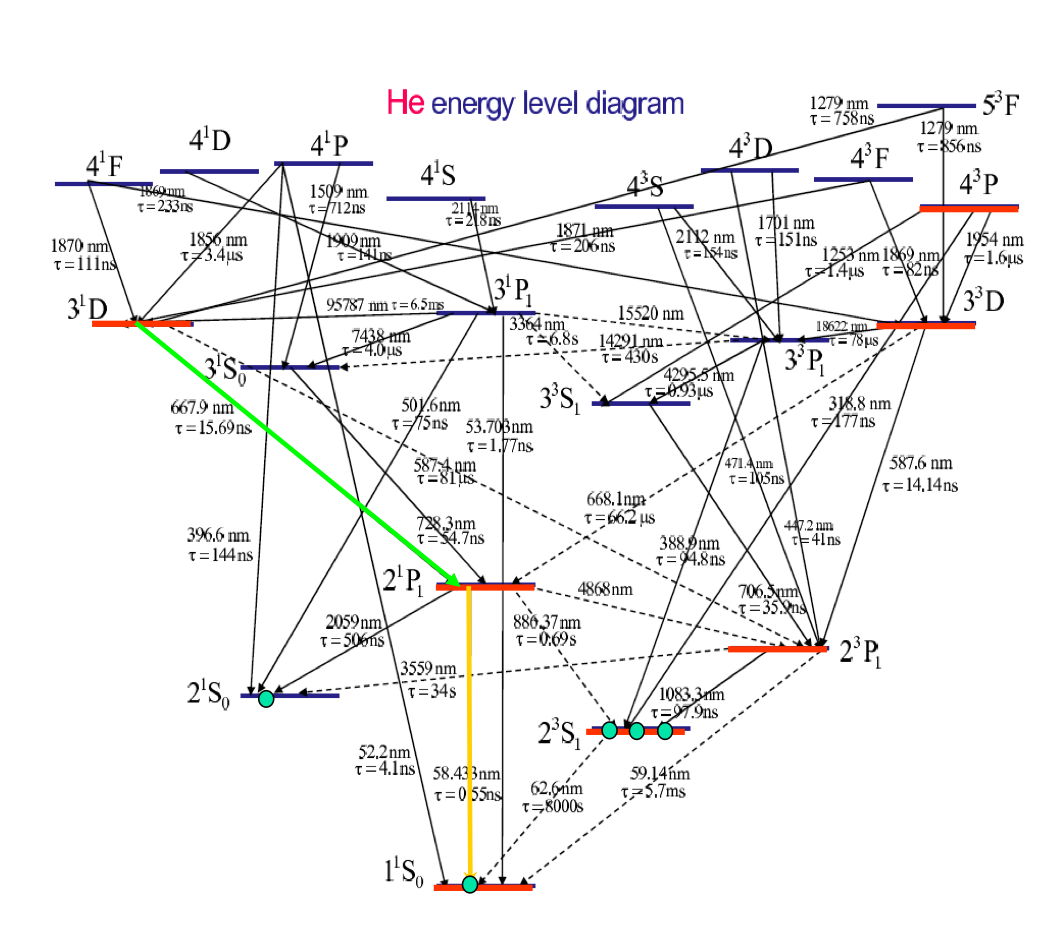
\includegraphics[width=0.9\linewidth]{ch-theory/figures/Helium_energy_levels}
    \caption[Sample Title Page Layout]{Helium energy levels~\cite{drake2007multiplet}}
    \label{fig:theory:HeEnergyLevel}
  \end{center}
\end{figure}



\chapter{Experiment\label{ch:experiment}}
\section{Apparatus}
Lasing system with a Ti:Sapphire amplifier lasing @ $800nm$, with a
pulse duration of $50ns$ and output energy of $3mJ$.

Optical parametric amplifier with a tunable wavelength wavelength
between $500nm ~ 2\mu m$, max energy is $100mJ$.
\section{Population probing techniques}
\subsection{Emission}
The first thing we want to study is probing the population at
different stages of ionized Helium. When you ionize Helium, the
electrons will recombine, cascaded down through collision to lower
state. So we want to know populations of certain level at certain
stage.

Several techniques have been developed to observe the behavior of this
ionized Helium.

The intense ionizing beam which is $800nm$ is focused to generate
ionized Helium and a plasma.
picture.

One of the emission lines of Helium which is dominating in visible, is
$587nm$.

Quantum weighs of triplet are 3 times bigger than singlet, so even the
A and B coefficient are similar, we see stronger lines.

Pressure broadening:
This is emission line at different pressure. The higher pressure you
have , the broader line width you will get.

Gated CCD spectra:
you record the spectra at different time of the Helium ionization, so
you get the dynamics of the emission of 587 lines, as a function of
time. From the spectrum, we could see that the peak occurs roughly at
$10ns$ after ionization. Besides, the width of the spectra is
shrinking as time goes by. The reason is that, after the ionization,
the density of the electron is high, and the width is due to collision
between electrons and atoms. As the plasma expand, you can see the
line gets narrower.

At different delay time, you can see different width of the spectra line.
\subsection{Transmission study}
Another technique is also developed to observe the population at
certain levels, by sending in a femto-second laser pulse, resonating
with one of the transitions.

One of the advantage of using femto-second laser is that it has very
wide spectrum, much wider than the transition itself.

So you could see absorption directly at the transmission spectra, of
the transmitted probe beam.

\subsection{Absorption vs Delay}
Typical spectra of femto-second pulse without ionizing Helium are 50fs
wide. As the time progress, you can see bigger and bigger effects of
the absorptio due to the accumulation of population of $2^3S$ over
time. This is done at fixed pressure.

\subsection{Absorption vs probe energy}
At different probing energy, you can see saturation effects because
depletion of population.

\subsection{linewidth as a function of pressure}
Another transition at $587nm$, which you also see this absorption
effects, we can carefully measure the line width at different
pressure.

Low pressure, it's linear, at higher pressure, because of saturation,
it's non-linear.

We have developed a method for probing the population evolution of
excited atoms, we are going to use this not only to measure the
population, but also linewidth, such as collision rates.

\section{Broadening Analysis}
Experiments show the line broadening of $587nm$ ($2^3P->3^3D$) is
$0.5nm$, while $1080nm$ ($2^3s->2^3P$), it's $0.4nm$

The Experiment Parameters are:
Helium: $200mbar$, the atom density is $5x10^{18}cm^{-3}$
Probe beam delay: $10ns$
Electron density: $2x10^{17}cm^{-3}$
Atom density(excited): $10^{14}cm^{-3}$
Electron temperature: $0.5eV$

For a rough estimation of electron-atom collision cross section, we
could use the equation as follows:
\begin{equation}
\sigma_{ea} = (n^2a_B)^2; \tau_{ea}=\frac{1}{N_e v_e \sigma_{ea}} =
212 ps (for 1.08 \mu m)
\end{equation}
picture.

There are different broadening mechanism:
- Natural: quite narrow, usually on the order of $1/1000$ $\Delta
\lambda_{collision}$, so could be neglected.
- Doppler: Due to thermal motion of the emitter.
- Instrumental: Equals to slit width times dispersion by grating.
- Collisional: When emitting, if the emitter colloided by other
particles, the emitting process will be disturbed.
- Other: Like the superradiance?

\subsection{Doppler Broadening}
\begin{equation}
\Delta w = 2 \sqrt{ln2} \sqrt{ \frac{2kT \lambda^2_0}{mc^2} }
\end{equation}

For $587nm$: $\Delta w_D = 0.32 nm$ while total is $5 \AA$.
For $1080nm$: $\Delta w_D = 0.59 nm$ while total is $24 \AA$.

So the Doppler broadening could be neglected.

\subsection{Instrumental Broadening}
Slit width: $40\mu m$

Instrumental broadening: $4 \AA$

Subtract instrumental from total:

587: $\sqrt{0.5^2-0.4^2} = 0.3 nm ~ 2.1 ps$

1080: $\sqrt{2.4^2-0.4^2} = 2.36 nm ~ 0.6 ps$

\subsection{Collisional Broadening}
Picture.

There's atom-atom collision and atom-election collision
(?electron-electron?)

But since the electron density ($10^{17}cm^{-3}$) is much higher than
atom density ($10^{14}cm^{-3}$), so the electron-atom collision will
dominate.

The weight of atoms are much higher than electrons, so atoms could not
gain much speed when laser present, while electron is fast!

Electron atom collision includes electron-impact excitation and
ionization, and their reverse processes, so one only need to consider
one of those processes.

Our electron is cold, only $0.5eV$, so the ionization cross section is
small, which could be neglected.

After the laser passed, it could be assumed that there's no photon, so
all photon related process like photo ionization/excitation could be
neglected.

Our electron density is high $10^{17}cm^{-3}$, so after laser passed,
electron reaches their local thermal equilibrium (LTE)(ref) quickly, at
$10ns$. Of course, Maxwellian distribution could be assumed.

To summarize, we just need to consider electron impact excitation,
under electron Maxwellian distribution.

From the Ralchenko paper(ref), we found the cross section fitting
curve, for electron impact transition between different states. This
curve is trustable, for it match experiments quite well.

The cross section is given by:
\begin{equation}
\sigma(E,\Delta E) = a_0^2 \pi \frac{R_y}{g_l E}
\Omega(\frac{E}{\Delta E})
\end{equation}
Where $a_0$ is just Bohr radius, $\pi a_0^2 = 0.8797 * 10^{-16} cm^2$,
$g_l$ is the statistical weight, for $2^3 S$ and $2^3 P$, $g_l = 3$.
$R_y = 13.6057 eV$ is the Rydberg energy. And $E$ is the collisional
energy, where $E=\frac{1}{2}mv^2$, $v$ could be calculated by
averaging through a Maxwellian distribution.

picture.

$\Delta E$ is the energy difference between initial and final states,
for $587nm$: it's $\frac{1.24}{0.587} eV$, while for $1080nm$, it's
$\frac{1.24}{1.08} eV$.

\begin{equation}
\Omega(x) = (A_1 ln(x) + A_2 + \frac{A_3}{x} + \frac{A_4}{x^2} +
\frac{A_5}{x^3}) (\frac{x+1}{x+A_6})
\end{equation}

For $2^3S -> 2^3P$, those coefficients are:

\begin{tabular}{ l | r }
  $A_1$ & $7.696 * 10^1$ \\
  $A_2$ & $1.250 * 10^2$ \\
  $A_3$ & $4.938 * 10^1$ \\
  $A_4$ & $-4.778 * 10^1$ \\
  $A_5$ & $3.189 * 10^2$ \\
  $A_6$ & $8.157$
\end{tabular}

While for $2^3S -> 2^3P$, those coefficients are:

\begin{tabular}{ l | r }
  $A_1$ & $1.414 * 10^2$ \\
  $A_2$ & $9.031 * 10^1$ \\
  $A_3$ & $-6.238 * 10^2$ \\
  $A_4$ & $1.183 * 10^3$ \\
  $A_5$ & $-6.424 * 10^2$ \\
  $A_6$ & $8.626$
\end{tabular}

So now we got everything to estimate $\sigma v$
\begin{equation}
\sigma(E,\Delta E) = \pi a_0^2 \frac{R_y}{g_l E}\Omega(\frac{E}{\Delta
E})
\end{equation}

Since we have Maxwellian distribution:
\begin{equation}
f(v) dv = (\frac{m}{2\pi k T})^(\frac{3}{2})4\pi v^2
exp(\frac{-mv^2}{2kT}) dv
\end{equation}

by switching to energy using, $E=\frac{1}{2}mv^2$, $v=\sqrt{2E}{m}, dv
=\frac{1}{\sqrt{2mE}}dE$, we got:
\begin{equation}
f(E)dE=(\frac{m}{2\pi k T})^{\frac{3}{2}}4\pi \frac{2E}{m} exp(-
\frac{E}{kT}) \frac{1}{\sqrt{2mE}} dE
\end{equation}
So we get:
\begin{equation}
<\sigma v> = \int_0^{+\inf} \sigma(E)\sqrt{\frac{2E}{m}}f(E)dE
\end{equation}
Then using,
\begin{equation}
\tau_{ea} = \frac{1}{N_e<\sigma v>}
\end{equation}
Where $N_e=2*10^{17}cm^{-3}$

By using Mathematica to compute the integral, it turns out that
$\tau_{ea}$ is quite small. This results is reasonable, for our
electron is cold, $kT=0.5eV$, this is small compared to $3^3D$ ->
$2^3P$ and $2^3P$ -> $2^3S$ gap, so the cross section should be small.

Picture.

However this is not the end of the story, this small result enlightens
us to focus on the electron-impact transition, whose cross section is
big in our case. Apparently, the smaller the energy difference,
between the initial and final state, the easier to excite, so the
cross section is bigger.

The total cross section is the sum of all the transitions, so let's
focus on the dominating one first.

For final state $3^3D$, the most close energy level is $3^1D$, and for
$2^3P$, it's $2^1P$. Now we look for the cross section of these two
transitions.

From graph 15 on page 617, $2^3P$ -> $2^1P$, cross section reads
$\sigma = 10^{-15}cm^2$ @ $0.5eV$

around $0.5eV$, the curve is flat enough to avoid taking average from
Maxwellian distribution.
\begin{equation*}
<v> = 2*10^7 cm/s
\end{equation*}
\begin{equation*}
<\sigma v> = \sigma <v>
\end{equation*}
\begin{equation}
\tau_{ea} = \frac{1}{N_e<\sigma v>} = \frac{1}{N_e \sigma <v>}
=\frac{1}{2*10^{17}cm^{-3}*10^{-15}cm^2*2*10^7cm/s} = 250 ps
\end{equation}

Similarly, by graph 28 on page 619, we found excitation from $3^3D$ ->
$3^1D$ dominates, whose cross section reads:
\begin{equation}
\sigma = 4.5 * 10^{-15} cm^2
\tau_{ea} = \frac{1}{N_e\sigma<v>} = 55ps
\end{equation}

But this could not explain all the broadening from experiments:

\begin{tabular}{ l c r }
       & Experiment & Calculation \\
  587  & 0.3nm(2.1ps) & 55ps \\
  1080 & 2.2nm(0.6ps) & 250ps \\
\end{tabular}

This indicates, there should be broadening factors brought in by other
effects. It should be superradiance. In that case, only the cylinder
of atoms contributes to superradiance, whose radius is $\lambda$, and
the length is plasma length.

Picture.

For 587nm, the single atom decay is given by:
\begin{equation}
\tau = \frac{1}{A} = 14ns
\end{equation}
The superradiance factor is:$N_a\lambda^2L/2\pi$, where
$N_a=10^{14}cm^{-3}$, $\lambda=587nm$, $L=0.7cm$, so the broadening
brought in by superradiance is:
\begin{equation}
\tau_s=\frac{\tau}{N_a\lambda^2L/2\pi} \\
= \frac{14ns}{10^{14}*0.587^2*10^{-8}*0.7/2\pi} = 0.364ps
\end{equation}
compared with $0.3ps$ experimental measurements, they are on the same
order.

For $1080nm$, $N_a$ is larger, and
\begin{equation}
\tau=\frac{1}{A}=100ns
\end{equation}
\begin{equation}
\tau_s=\frac{\tau}{N_a\lambda^2L/2\pi}=\frac{100ns}{4*10^{14}*1.08^2*0.7*10^{-8}/2\pi}=0.192ps
\end{equation}
While the width measured from experiment is $0.2ps$, they are on the
same order.

\section{Simulation Results}
If after ionization, a Maxwellian distribution could be assumed, it
will be quite handy. For only two parameters are needed to describe
the whole system. Otherwise, a more complicated method need to be take
to handle the distribution, like the code we are using, which traces
all the particles one by one.


\section{Superradiance}
\section{Carbon line identification}
%\section{Preliminary data and results on emission and absorption by excited Helium atoms}


%\section{Options}
\label{sec:usage:options}

In this section, we describe the options you can set when using this thesis class.
\tablespacing
% tablespacing is defined by the class to set single spacing for the long table when in doublespacing mode. If the singlespace option is set, this command has no effect.

\begin{longtable}{p{0.3\linewidth} p{0.6\linewidth}}

  % First page heading
  \caption[Options Provided by the PUthesis Class]{List of options for the puthesis document class and template} \label{tab:usage:options}\\
  \toprule
  \textbf{Option} & \textbf{Description} \\
  \midrule
  \endfirsthead

  % Future page heading
  \caption[]{(continued)}\\
  \toprule
  \textbf{Option} & \textbf{Description} \\
  \midrule
  \endhead

  % Page footer
  \midrule
  \multicolumn{2}{r}{(Continued on next page)}\\
  \endfoot

  % Last page footer
  \bottomrule
  \endlastfoot

  12pt &
  Specify the font size for body text as a parameter to \texttt{documentclass}. The Mudd Library requirements state that 12pt is preferred for serif fonts (e.g., Times New Roman) and 10pt for sans-serif fonts (e.g., Arial).
  \\

  letterpaper &
  If your document is coming out in a4paper, your LaTeX defaults may be wrong. Set this option as a parameter to \texttt{documentclass} to have the correct 8.5"x11" paper size.
  \\

  lot &
  Set this option as a parameter to \texttt{documentclass} to insert a List of Tables after the Table of Contents.
  \\


  lof &
  Set this option as a parameter to \texttt{documentclass} to insert a List of Figures after the Table of Contents and the List of Figures.
  \\

  los &
  Set this option as a parameter to \texttt{documentclass} to insert a List of Symbols after the Table of Contents and the other lists.
  \\

  singlespace &
  Set this option as a parameter to \texttt{documentclass} to single space your document. Double spacing is the default otherwise, and is required for the electronic copy you submit to ProQuest. Single spacing is permitted for the printed and bound copies for Mudd Library.
  \\

  draft &
  Set this option as a parameter to \texttt{documentclass} to have \LaTeX mark sections of your document that have formatting errors (e.g., overfull hboxes).
  \\

  % the cmidrule here spans both columns but is indented slightly on the left and right.
  \cmidrule[0.1pt](l{0.5em}r{0.5em}){1-2}

  \raggedright
  $\backslash newcommand$ $\{\backslash printmode\}\{\}$ &
  Insert this command after the \texttt{documentclass} command to turn off the hyperref package to produce a PDF suitable for printing.
  \\

  \raggedright
  $\backslash newcommand$ $\{\backslash proquestmode\}\{\}$  &
  Insert this command after the \texttt{documentclass} command to turn off the `colorlinks' option to the hyperref package. Links in the pdf document will then be outlined in color instead of having the text itself be colored. This is more suitable when the PDF may be viewed online or printed by the reader.
  \\

  $\backslash makefrontmatter$ &
  Insert this command after the \texttt{$\backslash begin\{document\}$} command, but before including your chapters to insert the Table of Contents and other front matter.
  \\

  \cmidrule[0.1pt](l{0.5em}r{0.5em}){1-2}

  $\backslash title$ &
  Set the title of your dissertation. Used on the title page and in the PDF properties.
  \\

  $\backslash submitted$ &
  Set the submission date of your dissertation. Used on the title page. This should be the month and year when your degree will be conferred, generally only January, April, June, September, or November. Check the Mudd Library rules~\cite{mudd2009} for the appropriate deadlines.
  \\

  $\backslash copyrightyear$ &
  Set the submission year of your dissertation. Used on the copyright page.
  \\

  $\backslash author$ &
  Your full name. Used on the title page, copyright page, and the PDF properties. \\

  $\backslash adviser$ &
  Your adviser's full name. Used on the title page. \\

  $\backslash departmentprefix$ &
  The wording that precedes your department or program name. Used on the title page. The default is ``Department of'', since most people list their department and can leave this out (e.g., Department of Electrical Engineering), however if yours is a program, set $\backslash departmentprefix\{Program in\}$ \\

  $\backslash department$ &
  The name of your department or program. Used on the title page. \\

  \cmidrule[0.1pt](l{0.5em}r{0.5em}){1-2}

  \raggedright
  $\backslash renewcommand$ $\{\backslash maketitlepage\}\{\}$ &
  Disable the insertion of the title page in the front matter. This is useful for early drafts of your dissertation. \\

  \raggedright  % full justification places the * in an awkward place
  $\backslash renewcommand*\{\backslash makecopyrightpage\}\{\}$ &
  Disable the insertion of the copyright page in the front matter. This is useful for early drafts of your dissertation. \\

  \raggedright
  $\backslash renewcommand*\{\backslash makeabstract\}\{\}$ &
  Disable the insertion of the abstract in the front matter. This is useful for early drafts of your dissertation. \\

\end{longtable}
\bodyspacing
% bodyspacing restores double spacing or single spacing after the table

% need blank space after \bodyspacing

I've seen other people print their dissertations using $\backslash pagestyle\{headings\}$, which places running headings on the top of each page with the chapter number, chapter name, and page number. This documentclass is not currently compatible with this option -- the margins are setup to be correct with page numbers in the footer, placing them 3/4" from the edge of the paper, as required. If you wish to use headings, you will need to adjust the margins accordingly.






\chapter{Conclusion\label{ch:conclusion}}

\input{ch-conclusion/conclusion} % Conclusion
\section{Future Work}
Syncronization with Thalas system.


 % Future work

\appendix % all chapters following will be labeled as appendices
\chapter{Appendicies\label{ch:appendicies}}

% Appendices are just chapters, included after the $\backslash appendix$ command.





%\chapter{Printing and Binding\label{ch:printing}}

\section{Printing}

For the library copies of your dissertation, you must use archival quality printing and binding. This means acid-free paper, containing at least 25\% cotton fiber. Triangle Repocenter on Nassau Street in Princeton offers both 25\% cotton paper and 100\% cotton paper. Most people choose the 25\% cotton paper, and this is generally recommended by the binders. The 100\% copy paper is somewhat thicker and the extra expense is unnecessary. 

Triangle offers online submission of your printing and binding order at: \url{http://triangleprinceton.com/collegiatebinding/thesis/}. If you request binding from them, they will deliver the paper copies to Smith-Shattuck Bookbinding for you and allow you to pick up the completed copies at their store on Nassau Street. The whole process takes 2-3 business days, but check with them in advance during the busy thesis-printing season in April and May. 

Currently, your printed and bound dissertation copies can be single spaced. Only the electronic copy submitted to ProQuest must be double spaced. All copies must be printed single-sided, with specific margins. 

\section{Binding}

An archival-quality sewn binding is required for the library copies of your dissertation. Smith-Shattuck Bookbinding is highly recommended, and is used by most students. Triangle Repocenter will send your copies there for you, greatly simplifying the process, but you can call Smith-Shattuck with special requests. 

The ``library standard'' sewn binding is sufficient for the copies to be sent to Mudd Library. It uses a black buckram cloth cover, which is the most popular option. For extra copies for yourself and your family members, you can choose ``buckram roundback binding'', which adds decorative lines on the spine, and printing of the title and author on the front cover. For a small additional fee, you can include the Princeton University shield on the front cover and a ribbon bookmark. Leather covers are also available. See Smith-Shattuck's website for more details at: \url{http://www.thesisbookbinding.com/}. 


%% Make the bibliography single spaced
\singlespacing
\bibliographystyle{plain}

%% add the Bibliography to the Table of Contents
\cleardoublepage
\ifdefined\phantomsection
  \phantomsection  % makes hyperref recognize this section properly for pdf link
\else
\fi
\addcontentsline{toc}{chapter}{Bibliography}

%% include your .bib file
\bibliography{lch-pums-thesis}

\end{document}

